\documentclass[11pt]{report}
\usepackage{titlesec}
\titleformat{\chapter}
  {\normalfont\LARGE\bfseries}{\thechapter}{1em}{}
\titlespacing*{\chapter}{0pt}{3.5ex plus 1ex minus .2ex}{2.3ex plus .2ex}

\usepackage[margin=1.2in]{geometry}
\usepackage[toc,page]{appendix}
\usepackage{graphicx}
\usepackage{lipsum}
\usepackage{caption}
\usepackage[utf8]{inputenc}
\usepackage[italian]{babel}
\usepackage{verbatim}
\usepackage{colorprofiles}
\usepackage{listings}   %<- per inserire il codice
\usepackage{float}
\usepackage{subcaption}
\usepackage{amsmath}
\usepackage{amsfonts}
\usepackage{listings}
\usepackage{xcolor}
\usepackage{url}
\usepackage{hyperref}


%%%%%%%%%%%%%%%%%%%%%%%%%%%%%%%%%%%%%%%%%%%%%%%%%%%%%%%%%%%%%%%%%%%%
\definecolor{custom_green}{rgb}{0,0.6,0}
\definecolor{codegray}{rgb}{0.5,0.5,0.5}
\definecolor{codepurple}{rgb}{0.58,0,0.82}
\definecolor{backcolour}{rgb}{0.95,0.95,0.92}
\definecolor{custom_blue}{rgb}{  0.05, 0.05, 0.97}
\definecolor{custom_brown}{rgb}{ 0.69, 0.38, 0.10}
\definecolor{custom_purple}{rgb}{0.58, 0.00, 0.82}
\definecolor{custom_orange}{rgb}{0.94, 0.59, 0.09}

\lstdefinestyle{MATLABstyle}{   
    commentstyle=\color{custom_green},
    keywordstyle=\color{magenta},
    numberstyle=\tiny\color{codegray},
    stringstyle=\color{codepurple},
    basicstyle=\ttfamily\footnotesize,
    breakatwhitespace=false,         
    breaklines=true,                 
    captionpos=b,                    
    keepspaces=true,                 
    numbers=left,                    
    numbersep=5pt,                  
    showspaces=false,                
    showstringspaces=false,
    showtabs=false,                  
    tabsize=2
}
\lstdefinelanguage{Cpp}{
      language=C++,
      backgroundcolor=\color{white},  
      basicstyle=\footnotesize \ttfamily \color{black} \bfseries,   
      breakatwhitespace=false,       
      breaklines=true,               
      captionpos=b,                   
      commentstyle=\color{custom_green},   
      deletekeywords={...},          
      escapeinside={\%*}{*)},
      keywordstyle=\color{custom_purple},
      identifierstyle=\color{blue},
      stringstyle=\color{blue},      
      numbers=left,                 
      numbersep=5pt,                  
      numberstyle=\tiny\color{black}, 
      rulecolor=\color{black},        
      showspaces=false,               
      showstringspaces=false,        
      showtabs=false,                
      stepnumber=1,                   
      tabsize=5,                     
      title=\lstname,                 
    }

\lstdefinelanguage{Python}{
    keywords={from, import, def, return, as, in, len, if, elif, else, for, while},
    breakatwhitespace=false,       
    breaklines=true,   
    morecomment=[l]{\#},
    morestring=[b]",
    commentstyle=\color{red},
    keywordstyle=\color{custom_purple},
    numberstyle=\tiny\color{black},
    stringstyle=\color{custom_green},
    basicstyle=\ttfamily\footnotesize,
    captionpos=b,
    showstringspaces=false,        
    showtabs=false,                
    numbers=left,                 
    numbersep=5pt,                  
    numberstyle=\tiny\color{black}, 
    rulecolor=\color{black},                      
    tabsize=5,                     
    title=\lstname,    
}

\lstdefinelanguage{MATLABc}{
    language=MATLAB,
    backgroundcolor=\color{white},  
    basicstyle=\footnotesize \ttfamily \color{black} \bfseries,   
    breakatwhitespace=false,       
    breaklines=true,               
    captionpos=b,
    morestring=[b]",
    commentstyle=\color{custom_green},   
    keywordstyle=\color{custom_blue},
    morekeywords={clearvars},
    deletekeywords={fprintf},
    identifierstyle=\color{black},
    stringstyle=\color{custom_purple},      
    numbers=left,                 
    numbersep=5pt,                  
    numberstyle=\tiny\color{black}, 
    rulecolor=\color{black},        
    showspaces=false,               
    showstringspaces=false,        
    showtabs=false,                
    stepnumber=1,                   
    tabsize=5,                     
    title=\lstname,                 
}
%%%%%%%%%%%%%%%%%%%%%%%%%%%%%%%%%%%%%%%%%%%%%%%%%%%%%%%%%%%%%%%%%%%%




\begin{document}
\captionsetup[figure]{margin=1.5cm,font=small,labelfont={bf},name={Figure},labelsep=colon,textfont={it}}
\captionsetup[table]{margin=1.5cm,font=small,labelfont={bf},name={Table},labelsep=colon,textfont={it}}


\begin{titlepage}
\begin{center}
\LARGE {\scshape{Università Politecnica delle Marche}}\\[0.5cm]
\LARGE {\scshape{Ingegneria Informatica e dell'Automazione}}\\[0.7cm]
\linespread{1}
\huge {\bfseries RoboSimCloth}\\[1cm]
\linespread{1}

\includegraphics[width=5cm]{images/logoUnivpm.jpg}\\[0.5cm]
\linespread{1.2}
\Large Corso di\\
\Large {\scshape{Laboratorio di Automazione}} \\[0.3cm]
\Large {Anno accademico 2024-2025 \\[0.8cm]}
{\Large Studenti:}
\hfill {\Large Professore:}\\
{\Large Pizzuto Andrea}
\hfill
{\Large Andrea Bonci}

\raggedright{\Large Meloccaro Lorenzo\\
\Large Percipalle Noemi\\} 



\raggedleft{\Large Dottorandi:\\
\Large Serafini Andrea\\
\Large Pellicani Ilaria\\
\Large Di Biase Alessandro\\[0.5cm]}
\centering{

\includegraphics[width=2cm]{images/dii_new.png}\\[0.3cm]
\large Dipartimento di Ingegneria dell'Informazione\\[0.3cm]
}
\end{center}
\end{titlepage}

\pagenumbering{arabic}
\tableofcontents
%\addcontentsline{toc}{chapter}{Introduzione}
\newpage

\pagestyle{plain}

\newpage
\chapter{Introduzione}
\textit{Il capitolo fornisce una panoramica del progetto, descrivendo l'obiettivo principale di sviluppare e simulare la movimentazione di un robot TM-900 con un tessuto, attraverso l'integrazione di ROS2 e Unity. Viene fornita una panoramica delle motivazioni per l'uso di questi software e delle principali fasi del progetto.}
\vspace{0.5cm}
\newline
Il presente progetto ha come obiettivo lo sviluppo e la simulazione della manipolazione dei tessuti con il robot collaborativo TM5-900, utilizzando l'integrazione di software avanzati come ROS2 e Unity. Il contesto applicativo del progetto si colloca nell'ambito industriale e robotico, ponendo particolare attenzione sull'ottimizzazione dei processi di smantellamento di oggetti deformabili, come abiti e tessuti. L'azienda coinvolta utilizza il software Cloth 3D per la modellazione degli abiti, mentre Unity e Gazebo sono impiegati per simulare la movimentazione del robot e l'interazione con gli oggetti.
Uno degli obiettivi di questo progetto è quello di analizzare in dettaglio l'integrazione tra ROS2 e Unity, scelta motivata dalle potenzialità di questi due strumenti. ROS2 offre una gestione efficiente della comunicazione tra il robot e il sistema di simulazione, mentre Unity fornisce la possibilità di simulare l'effetto della gravità sui tessuti e i movimenti del robot in tempo reale tramite una grafica avanzata. L'integrazione di questi due software è stata scelta per soddisfare la necessità di creare un ambiente simulativo realistico, utile non solo per eseguire test simulativi, ma anche per implementare successivamente il sistema su un robot reale.
In questo modo, l'integrazione tra ROS2 e Unity consente di gestire il robot e simularlo in ambiente virtuale, migliorando l'efficienza e la precisione nelle operazioni robotiche. Il progetto affronta diversi task, tra cui la valutazione e la compatibilità dei tessuti con i vari software, la simulazione della movimentazione del robot e dell'oggetto da disassemblare in un ambiente condiviso, l'acquisizione e la definizione di una sequenza di fasi di smantellamento, l'esecuzione delle fasi in simulazione con il robot e, infine, l'esecuzione delle stesse fasi su un robot reale.
% Spiegazione dettagliata del task assegnato al gruppo (cosa avete fatto e su quale sistema).\\
% Se per lo svolgimento del task è stato necessario interagire con altri gruppi che hanno lavorato sullo stesso sistema presentare anche brevemente i task svolti dagli altri gruppi e spiegare la loro interconnessione.
% Se si è invece optato per far confluire il lavoro di più gruppi in un'unica relazione, va spiegato qual era il task iniziale dei singoli gruppi e poi come è avvenuta l'integrazione. \\
% In sintesi, l'introduzione deve permettere al lettore di capire subito su cosa avete lavorato.
% Al termine dell'introduzione inserite anche una breve descrizione per capitoli del contenuto della restante parte della relazione (es Nel Capitolo \ref{Hardware} viene descritto...). \\
% \newline
% Nel seguito la struttura in capitoli di massima per ogni relazione, da adattare qualora necessario. \\
% \textcolor{red}{NOTA: La relazione va pensata e scritta nell'ottica di dare a chi verrà dopo di voi un documento utile per capire a che punto è arrivata l'attività svolta dal vostro gruppo e per metterli in condizione di portare avanti il vostro lavoro. Di conseguenza dovete essere chiari e diretti, riportando solo le informazioni necessarie e evidenziando in modo critico cosa effettivamente funziona correttamente e cosa va migliorato}

\newpage
\chapter{Materiali e Metodi}
\textit{In questo capitolo saranno presentati i materiali(hardware e software) e i metodi, quindi le tecniche utilizzate, inoltre vengono dettagliate le tecnologie impiegate e le procedure seguite, in modo da permettere la riproducibilità del progetto. In particolare la prima sezione, \textbf{Hardware} comprende la descrizione del robot utilizzato in simulazione Omron TM5-900 e della camera RealSense D435i. Successivamente saranno presentati i vari \textbf{Software}, utilizzati all'interno del progetto e che hanno permesso la riuscita dell'applicazione, tra i quali Ubuntu, ROS2, Moveit, Gazebo, Unity e in particolare lo strumento Cloth di Unity. Infine, verranno descritte nel dettaglio la \textbf{Predisposizione dei Software} nel PC e le modalità di \textbf{Interfacciamento tra ROS 2 e Unity}, con focus su strumenti fondamentali come ROS-TCP Connector, ROS-TCP Endpoint e URDF Importer.}

\section{Hardware}
\textit{In questa sezione verranno presentati i principali componenti hardware utilizzati nel progetto, in particolare il robot Omron TM5-900 e la Stereo-Camera RealSense D435i. Saranno forniti dettagli tecnici e funzionali su ciascun componente, evidenziando le loro caratteristiche principali e il loro ruolo all'interno del sistema di simulazione.}

\subsection{Omron TM5-900}
\begin{figure}[h!]
    \centering
    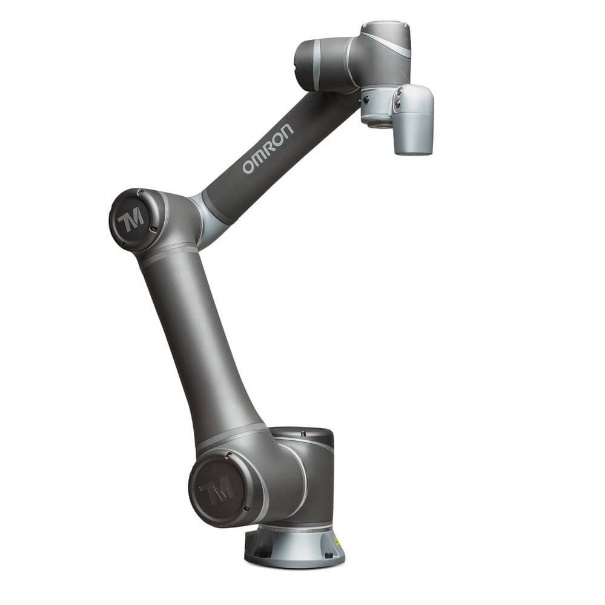
\includegraphics[width=0.6\textwidth]{images/omron.png}
    \caption{Omron TM5-900}
    \label{fig:omron}
\end{figure}

Un robot è un manipolatore riprogrammabile e multifunzionale progettato per spostare materiali, parti, strumenti o dispositivi specializzati attraverso vari movimenti programmati per l'esecuzione di una varietà di compiti. Il \textbf{robot OMRON TM5-900} è un robot industriale collaborativo (cobot) di ultima generazione, progettato per applicazioni che richiedono flessibilità, precisione e la capacità di operare in ambienti dinamici e collaborativi. È dotato di una serie di caratteristiche avanzate che lo rendono adatto a una varietà di compiti in ambienti industriali, inclusi il montaggio, il pick-and-place, e operazioni di smontaggio come quelle previste in questo progetto.

Tra le caratteristiche principali vi sono:

\begin{itemize}
    \item \textbf{Design compatto e flessibile}: Il TM5-900 è progettato per lavorare in spazi ristretti, con un braccio robotico che può essere facilmente integrato in linee di produzione esistenti senza necessitare di ampi spazi operativi. La sua flessibilità gli consente di essere facilmente usato per diverse applicazioni.
    \item \textbf{Portata e capacità di carico}: Il TM5-900 ha una capacità di carico utile fino a 5 kg, che lo rende adatto a manipolare una varietà di oggetti e strumenti, come i tessuti utilizzati in questo progetto.
    \item \textbf{Gradi di libertà (DOF)}: Il TM5-900 è dotato di 6 gradi di libertà (DOF), che gli consentono di eseguire movimenti complessi e articolati, simili a quelli di un braccio umano. Questo permette al robot di raggiungere e manipolare oggetti in spazi tridimensionali con alta precisione.
    \item \textbf{Giunti e movimenti}: Il robot è equipaggiato con giunti motorizzati, che consentono di controllare i movimenti di rotazione in modo fluido e preciso. I giunti, insieme ai sensori di forza e coppia, permettono di eseguire operazioni delicate, come il manipolamento di oggetti morbidi (ad esempio i tessuti) senza danneggiarli.
    \item \textbf{Facilità di programmazione e utilizzo}: Questo robot è dotato di un'interfaccia utente intuitiva e di software di programmazione che ne facilita l'uso anche da parte di personale non specializzato. La programmazione è resa semplice grazie alla modalità di "teaching", che consente di insegnare al robot i movimenti direttamente sul campo.
    \item \textbf{Tecnologia di sensori avanzati}: Il TM5-900 è equipaggiato con sensori di forza e coppia, che permettono di eseguire operazioni delicate con una precisione millimetrica, ideale per manipolare oggetti senza danneggiarli.
    \item \textbf{Compatibilità con ROS2}: Il robot è compatibile con il sistema ROS2, che consente di integrarlo facilmente in ambienti di simulazione come Gazebo e Unity, come previsto nel progetto. Questo permette di controllare il robot tramite comandi remoti e di simulare il suo comportamento in ambienti virtuali.
\end{itemize}

In questo progetto, il robot OMRON TM5-900 è stato scelto per la sua versatilità e capacità di manipolare oggetti come tessuti in modo preciso e sicuro. Il suo utilizzo si concentra sulla simulazione della movimentazione del robot, dove l'integrazione con ROS2 assicura una gestione ottimale della comunicazione e delle operazioni. Inoltre, l'interazione con Unity permette di visualizzare in tempo reale il comportamento del robot, monitorando e ottimizzando il suo funzionamento durante le diverse fasi del progetto.

\subsection{Stereo-Camera RealSense D435i}

\section{Software}
\textit{In questo capitolo verranno analizzati i software principali utilizzati per il progetto: Ubuntu, Robot Operating System 2, Moeveit, Gazebo e Unity. Verranno fornite una panoramica generale, informazioni sul loro utilizzo e sulle versioni adottate. Inoltre, si approfondirà l'uso del componente Cloth di Unity, che ha rivestito un ruolo centrale nella simulazione della fisica dei tessuti.}

\subsection{Ubuntu}

\subsection{Robot Operating System 2}

\begin{figure}[H]
    \centering
    
\includegraphics[width=0.6\textwidth]{images/ROS2.png}
    \caption{Logo ROS2}
    \label{fig:ROS2}
\end{figure}

\textbf{ROS 2} (Robot Operating System 2) \cite{ROS2} è un framework open-source per lo sviluppo di applicazioni robotiche. Fornisce una serie di strumenti, librerie e convenzioni per facilitare la comunicazione tra i componenti software di un sistema robotico. ROS 2 è progettato per migliorare la scalabilità, la sicurezza e la compatibilità con i sistemi distribuiti rispetto al suo predecessore, ROS 1. Il suo utilizzo è diffuso in ricerca e industria per il controllo di robot mobili, bracci robotici e veicoli autonomi.
In questo progetto, ROS 2 è stato utilizzato per gestire la comunicazione tra il robot simulato in Unity e i componenti di controllo. ROS 2 permette lo scambio di messaggi tra i nodi, abilitando il controllo del robot da Unity e viceversa. In particolare, il framework ha permesso l'integrazione con il sistema di simulazione, la gestione delle traiettorie e il controllo dei giunti del manipolatore.
Inizialmente, il progetto è stato avviato con ROS 2 Jazzy, ma si sono riscontrati diversi problemi di compatibilità e instabilità, in particolare con l'integrazione del ROS-TCP Connector per Unity. Per questo motivo, è stato deciso di passare a ROS 2 Humble, una versione più stabile e ampiamente supportata, che ha garantito una migliore compatibilità con gli strumenti di sviluppo utilizzati.

\subsection{Moveit}

\subsection{Gazebo}

\subsection{Unity e UnityHUB}

\begin{figure}[h!]
    \centering
    
\includegraphics[width=0.6\textwidth]{images/UNITY.jpg}
    \caption{Logo Unity}
    \label{fig:UNITY}
\end{figure}

Unity \cite{Unity} è un motore di gioco e simulazione ampiamente utilizzato per la creazione di ambienti interattivi in tempo reale. Sebbene sia nato per lo sviluppo di videogiochi, il suo utilizzo si è esteso ad applicazioni di simulazione, robotica, realtà virtuale e aumentata. Unity permette di creare ambienti 3D realistici e interattivi grazie al suo motore grafico avanzato e alle sue funzionalità di scripting basate su C\#.
In questo progetto, Unity è stato utilizzato come ambiente di simulazione per il robot. Grazie alla sua compatibilità con ROS2 tramite il ROS-TCP Connector, Unity ha permesso di visualizzare il robot, simulare i suoi movimenti e interagire con l'ambiente circostante. Il motore fisico di Unity è stato sfruttato soprattutto per replicare le dinamiche fisiche della maglietta, garantendo una simulazione più realistica delle interazioni tra un indumento e gli oggetti della scena.
Per lo sviluppo del progetto, abbiamo utilizzato Unity 6, la versione più recente al momento di sviluppo del progetto.

\subsection{Strumento Cloth di Unity}
Il sistema \textbf{Cloth di Unity} offre una soluzione basata sulla fisica per simulare tessuti e materiali flessibili all'interno di ambienti 3D. Sebbene sia stato progettato principalmente per rappresentare abbigliamento su personaggi, può essere utilizzato anche per altri scopi, come bandiere, tende o qualsiasi altro oggetto che richieda una simulazione realistica del comportamento dei tessuti\cite{ManualCloth}.
In questo progetto, il componente Cloth riveste un ruolo centrale, poiché il compito finale prevede che l'indumento manipolato dal robot presenti una fisica il più possibile realistica, simulando accuratamente il comportamento del tessuto. A tal fine, sono stati forniti tre file principali relativi a una maglietta: un file \textbf{OBJ}, un file \textbf{FBX} e un file \textbf{Collada}. 
L'analisi di questi file ha permesso di ottenere informazioni utili riguardo al formato da utilizzare e alle caratteristiche della mesh per applicare efficacemente il componente Cloth.
\newline
Tra la documentazione di Unity è possibile trovare anche quella relativa al componente Cloth e in seguito verranno riassunti i passaggi fondamentali per utilizzarlo al meglio.
Per implementare una simulazione di tessuto in Unity, è necessario aggiungere il componente Cloth a un oggetto mesh. Ecco i passaggi fondamentali:
\begin{itemize}
    \item \textbf{Preparazione della Mesh}: è importante assicurarsi che l'oggetto a cui si desidera applicare il tessuto abbia una mesh adeguata, e quindi, come visto in precedenza, anche un numero adeguato di poligoni della mesh.
    
    \item \textbf{Aggiunta del Componente}: una volta importato il file su Unity è sufficiente selezionare l'oggetto nella gerarchia di Unity e, nel pannello Inspector, cliccare su "Add Component", selezionare "Physics" e poi "Cloth" dalla lista dei componenti disponibili.

    \item \textbf{Configurazione}: Una volta aggiunto il componente, sarà possibile modificare vari parametri per ottenere una simulazione personalizzata e accurata.
\end{itemize}

Affinchè la maglietta abbia una movimentazione guidata dalla fisica, deve chiaramente avere una parte della maglietta fissata e che quindi non è soggetta alla gravità. Questi su Unity vengono chiamati "Cloth Constraint" e quindi "vincoli del Cloth".
Di seguito una descrizione dei passaggi per applicarli correttamente alla maglietta:
\begin{enumerate}
    \item sul componente Cloth si clicca su "Edit Cloth Constraint" come possiamo vedere dalla figura \ref{fig:cloth_constraints}
    \begin{figure}[h!]
        \centering
        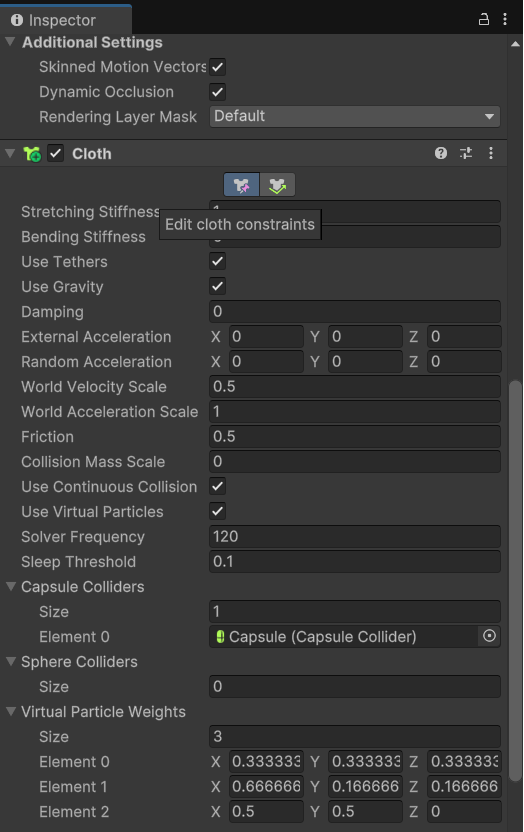
\includegraphics[width=0.3\textwidth]{images/cloth_constraints.PNG}
        \caption{Schermata Unity per l'applicazione dei vincoli}
        \label{fig:cloth_constraints}
    \end{figure}
    \item successivamente si aprirà una schermata che permetterà di selezionare (tramite "Select") oppure colorare (tramite "Paint") le parti che saranno vincolate e quindi rimarranno maggiormente rigide. E' importante specificare una distanza minima nel parametro "Max Distance", in figura \ref{fig:cloth_constraints_2} è stato assegnato il valore 0.2 ed ha permesso un buon risultato.
    \begin{figure}[h!]
        \centering
        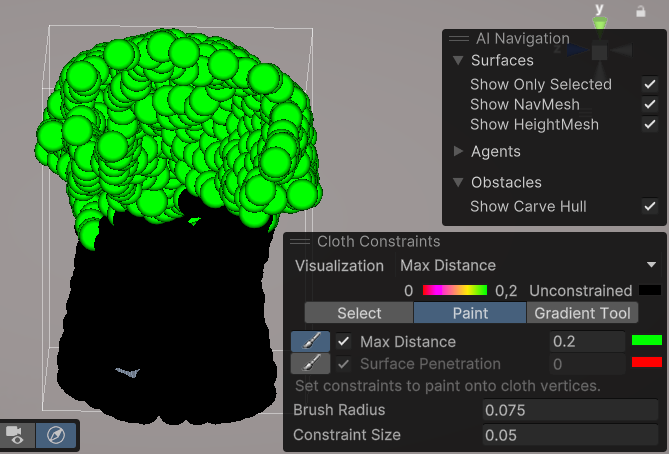
\includegraphics[width=0.5\textwidth]{images/cloth_constraints_2.PNG}
        \caption{Schermata Unity per la selezione delle parti della mesh a cui applicare i vincoli}
        \label{fig:cloth_constraints_2}
    \end{figure}
\end{enumerate}



Infine una descrizione delle principali proprietà del componente Cloth e di come sono state utilizzate nell'implementazione del tessuto realistico della maglietta:
\begin{itemize}
    \item \textbf{Stretching Stiffness}: Determina la resistenza del tessuto all'allungamento. Valori più alti rendono il tessuto meno incline a estendersi. Un parametro accettabile per la maglietta è risultato compreso tra 0,5 e 0,7.

    \item \textbf{Bending Stiffness}: Controlla la rigidità alla flessione del tessuto. Un valore elevato riduce la capacità del tessuto di piegarsi. Un parametro accettabile per la maglietta è risultato compreso tra 0,7 e 0,9.

    
    \item \textbf{Use Tethers}: Applica vincoli che aiutano a prevenire che le particelle mobili del tessuto si allontanino troppo da quelle fisse, riducendo l'eccessiva elasticità.
    
    \item \textbf{Use Gravity}: Indica se la gravità deve influenzare il tessuto. Da applicare nel caso in cui si voglia vedere una movimentazione fisica della maglietta e condizionata dalla gravità.
    
    \item \textbf{Damping}: Coefficiente che determina quanto velocemente il movimento del tessuto si smorza nel tempo.  Un parametro accettabile per la maglietta è risultato compreso tra 0,2 e 0,4.
    
    \item \textbf{External Acceleration}: Applica un'accelerazione costante esterna al tessuto, utile per simulare effetti come il vento.
    
    \item \textbf{Random Acceleration}: Introduce un'accelerazione casuale al tessuto, aggiungendo variazioni imprevedibili nel movimento.
    
    \item \textbf{World Velocity Scale}: Determina quanto il movimento in spazio globale dell'oggetto influisce sui vertici del tessuto.
    
    \item \textbf{World Acceleration Scale}: Controlla l'influenza dell'accelerazione globale dell'oggetto sui vertici del tessuto.
    
    \item \textbf{Friction}: Imposta il coefficiente di attrito del tessuto durante le collisioni.  Un parametro accettabile per la maglietta è risultato compreso tra 0,5 e 0,7.
    
    \item \textbf{Collision Mass Scale}: Determina l'incremento di massa delle particelle durante le collisioni.
    
    \item \textbf{Use Continuous Collision}: Abilita la collisione continua per migliorare la stabilità delle interazioni.
    
    \item \textbf{Use Virtual Particles}: Aggiunge particelle virtuali per migliorare la stabilità delle collisioni.
    
    \item \textbf{Solver Frequency}: Specifica il numero di iterazioni del solver per secondo, influenzando la precisione della simulazione. Un parametro accettabile per la maglietta è risultato 60 Hz.
    
    \item \textbf{Sleep Threshold}: Definisce la soglia sotto la quale il tessuto entra in stato di "sonno", interrompendo la simulazione fino a nuove interazioni. Un parametro accettabile per la maglietta è risultato 0,1. 
    
    \item \textbf{Capsule Colliders}: Array di collisori a capsula con cui il tessuto può interagire.
    
    \item \textbf{Sphere Colliders}: Array di coppie di collisori sferici con cui il tessuto può interagire.
\end{itemize}



% \section{Componente1}
% \section{Componente2}
% \section{Schema dei collegamenti}
% Inserire uno schema dei collegamenti analogo a quello in Figura \ref{fig:schema}. Si suggerisce per lo scopo di usare il software "draw.io". Nello schema riportare tutti i collegamenti tra i componenti, specificando quale pin di un componente1 si collega con quale pin di un componente2 (per la maggior parte dei collegamenti dovete cioè avere una linea con 2 label). \\
% Inserire anche una descrizione testuale dello schema.

% \begin{figure}[H]
% \centering
% 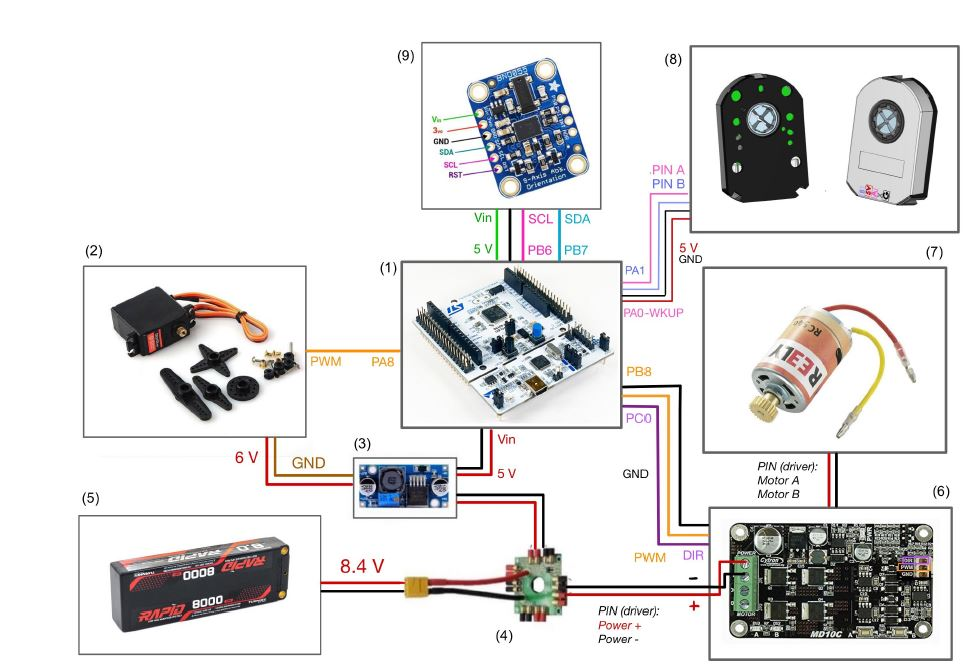
\includegraphics[width=0.8\textwidth,keepaspectratio]{figures/Schema.JPG}
% \caption{Schema dei collegamenti}
% \label{fig:schema}
% \end{figure}

\section{Predisposizione dei Software nel PC}

\section{Interfacciamento ROS2-Unity}

\subsection{ROS-TCP Connector \& ROS-TCP Endpoint}
Il \textbf{ROS-TCP Endpoint} è il nodo ROS2 complementare al \textbf{ROS-TCP Connector}, che permette a Unity di comunicare con ROS tramite la rete. Questo nodo gestisce le connessioni TCP in ingresso provenienti da Unity e inoltra i messaggi ROS corrispondenti ai topic.

\section*{\textbf{Installazione del ROS-TCP Endpoint}}
Per utilizzare il \textbf{ROS-TCP Endpoint}, è necessario installarlo all'interno del proprio workspace ROS2:

\begin{itemize}
    \item \textbf{Clonare il repository}: \texttt{cd ~/tuo\_workspace/src}
    \item \textbf{Compilare il workspace}: \texttt{cd ~/tuo\_workspace}
    \begin{verbatim}
    colcon build --symlink-install
    source install/setup.bash
    \end{verbatim}
\end{itemize}

\section*{\textbf{Avvio del nodo}}

Per avviare il nodo \textbf{ros\_tcp\_endpoint}, bisogna eseguire il comando:

\begin{verbatim}
ros2 launch ros_tcp_endpoint endpoint.launch.py
\end{verbatim}

In questo modo si avvia il server che ascolta sulla porta TCP (di default 10000) per ricevere le connessioni da Unity.

\subsection*{\textbf{Verifica del nodo}}
Per assicurarsi che il nodo sia in esecuzione, è possibile utilizzare il comando: \begin{verbatim}
ros2 node list
\end{verbatim}

In questo modo il nodo \textbf{/ros\_tcp\_endpoint\_node} dovrebbe essere visibile nella lista.

\subsection*{\textbf{Verifica della connessione}}

Per testare la connessione tra Unity e ROS2 bisogna:

\begin{itemize}
    \item \textbf{1.} Avviare ROS2 ed eseguire il nodo \texttt{ros\_tcp\_endpoint}.
    \item \textbf{2.} Eseguire la simulazione in Unity e verificare che non vengano generati errori di connessione.
    \item \textbf{3.} Utilizzare \texttt{ros2 topic echo} per controllare i messaggi pubblicati da Unity verso ROS2 e viceversa.
\end{itemize}

Questa configurazione permette di integrare Unity e ROS2 in un ambiente di simulazione realistico, abilitando lo scambio di dati tra il motore grafico e il framework robotico per la pianificazione e il controllo dei movimenti.

\subsection*{\textbf{ROS-TCP Connector}}

Il \textbf{ROS-TCP Connector} è un pacchetto sviluppato da Unity Technologies che permette di mettere in comunicazione ROS2 e Unity attraverso una connessione TCP. Questa integrazione è fondamentale perché consente di inviare e ricevere messaggi tra i due ambienti, facilitando lo sviluppo e la simulazione di robot. Grazie a questo pacchetto, Unity diventa un ambiente in cui è possibile visualizzare i dati provenienti da ROS2, testare il controllo e verificare il comportamento del robot in scenari simulati prima di passare alla fase di implementazione su un sistema reale.

Il pacchetto ROS-TCP Connector include:

\begin{itemize}
    \item \textbf{ROS-TCP Connector}: permette l’invio e la ricezione di messaggi tra Unity e ROS2.
    \item \textbf{VISUALIZATIONS PACKAGE}: utile per la visualizzazione dei messaggi in entrata e in uscita nella scena di Unity, facilitando il debug e l'analisi dei dati.
\end{itemize}

Inoltre, il pacchetto offre diverse funzionalità:

\begin{itemize}
    \item \textbf{ROSConnection}: gestisce l’intero processo di comunicazione tra Unity e ROS2.
    \item \textbf{Message Generation}: permette di generare automaticamente classi in C\# che rappresentano i messaggi ROS2, facilitando l’interazione tra i due ambienti.
    \item \textbf{Visualizations}: un set di API e configurazioni predefinite per rappresentare le informazioni scambiate.
    \item \textbf{ROSGeometry}: una serie di estensioni utili per la conversione delle geometrie tra Unity e altri sistemi che semplificano la compatibilità tra gli ambienti di simulazione.
\end{itemize}

\subsection*{\textbf{Installazione del ROS-TCP Connector}}

Per utilizzare il ROS-TCP Connector, è necessario installarlo all’interno di Unity e configurarlo correttamente affinché possa dialogare con ROS2.

Il pacchetto è disponibile su GitHub e può essere importato in Unity tramite il Package Manager. Ecco come fare:

\begin{itemize}
    \item Aprire Unity e accedere al menu "Window", poi selezionare "Package Manager".
    \begin{figure}[h]
        \centering
        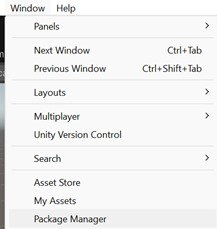
\includegraphics[width=0.4\textwidth]{images/rostcp.jpg}
        \caption{Package Manager in Unity}
        \label{fig:rostcp}
    \end{figure}
    
    \item Nella finestra del Package Manager, cliccare sul pulsante “+” in alto a sinistra e selezionare "Add package from git URL...".
    \begin{figure}[h]
        \centering
        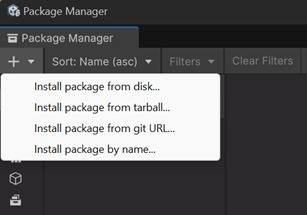
\includegraphics[width=0.4\textwidth]{images/rostcp1.jpg}
        \caption{Package Manager in Unity}
        \label{fig:rostcp1}
    \end{figure}

    \item Inserire l’URL del pacchetto da installare:
    \begin{itemize}
        \item \textbf{ROS-TCP Connector}: 
        \url{https://github.com/Unity-Technologies/ROS-TCP-Connector.git?path=/com.unity.robotics.ros-tcp-connector}
        \item \textbf{Visualizations Package}: 
        \url{https://github.com/Unity-Technologies/ROS-TCP-Connector.git?path=/com.unity.robotics.visualizations}
    \end{itemize}
    
    \item In alternativa, se si ha una copia locale del pacchetto, è possibile installarlo seguendo la guida ufficiale di Unity per l’installazione di pacchetti locali.
\end{itemize}

\subsection*{\textbf{Configurazione del ROS-TCP Connector}}

Dopo aver installato il pacchetto, è necessario configurarlo per far sì che possa comunicare con ROS2. Questo passaggio è essenziale per garantire che Unity e ROS2 possano scambiarsi dati senza problemi.

Dopo aver caricato l’oggetto, per configurare la comunicazione, bisogna:

\begin{itemize}
    \item Accedere al menu "Robotics" e selezionare "ROS Settings".
    \begin{figure}[H]
        \centering
        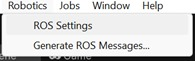
\includegraphics[width=0.4\textwidth]{images/rostcp2.jpg}
        \caption{Menu "Robotics" e "ROS Settings"}
        \label{fig:rostcp2}
    \end{figure}
    
    \item Nel campo "ROS IP Address", inserire l'indirizzo IP della macchina su cui è in esecuzione ROS2.
    \begin{figure}[H]
        \centering
        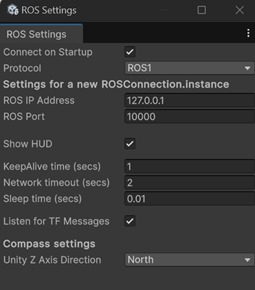
\includegraphics[width=0.4\textwidth]{images/rostcp4.jpg}
        \caption{Configurazione dell'indirizzo IP di ROS2}
        \label{fig:rostcp4}
    \end{figure}
\end{itemize}

Per reperire l'indirizzo IP di ROS (ROS IP Address) sulla macchina con WSL, è sufficiente aprire un terminale e digitare:

\begin{verbatim}
hostname -I
\end{verbatim}

\subsection*{\textbf{Comunicazione tra ROS2 e Unity}}

Dopo aver completato l’installazione e la configurazione, Unity sarà in grado di comunicare con ROS2 attraverso il protocollo TCP. Questo avviene tramite due modalità principali:

\begin{itemize}
    \item \textbf{Pubblicazione di Messaggi}: Unity può inviare dati a ROS2 utilizzando il componente \texttt{ROSPublisher}.
    \item \textbf{Sottoscrizione di Messaggi}: Unity può ricevere dati da ROS2 grazie al componente \texttt{ROSSubscriber}.
\end{itemize}

Per rendere tutto operativo, è necessario avviare il nodo \texttt{ros\_tcp\_endpoint} all’interno di ROS2. Questo nodo funge da intermediario e garantisce che i messaggi possano fluire correttamente tra i due sistemi.

\subsection*{\textbf{Testare la connessione tra Unity e ROS2}}


Una volta configurata la comunicazione, è importante verificare che tutto funzioni correttamente. Ecco alcuni passaggi per effettuare un controllo:

\begin{itemize}
    \item \textbf{1. Avviare ROS2 ed eseguire il nodo \texttt{ros\_tcp\_endpoint}.}
    \item \textbf{2. Digitare il comando per configurare l'ambiente ROS:}
    \begin{verbatim}
    source ~/tuo_workspace/install/setup.bash
    \end{verbatim}
    \item \textbf{3. Avviare il nodo tramite il comando:}
    \begin{verbatim}
    ros2 launch ros_tcp_endpoint endpoint.launch.py
    \end{verbatim}
    Questo avvierà il nodo \texttt{ROS-TCP Endpoint}, che ascolterà le connessioni da Unity sulla porta 10000 (di default).
    \item \textbf{4. È possibile verificare se il nodo è in esecuzione tramite il comando:}
    \begin{verbatim}
    ros2 node list
    \end{verbatim}
\end{itemize}


\subsection{Eseguire simulazione in Unity}
\begin{itemize}
    \item Utilizzare il comando \texttt{ros2 topic echo} per verificare se i messaggi vengono effettivamente inviati e ricevuti tra Unity e ROS2.
\end{itemize}

Se tutto è stato configurato correttamente, Unity e ROS2 saranno perfettamente integrati e potranno scambiarsi dati in tempo reale.

Per concludere, grazie a questa configurazione, sarà possibile avere uno scambio di dati per la pianificazione e il controllo dei movimenti.

\subsection{URDF Importer}

L'\textbf{URDF Importer} \cite{URDF-Importer} di Unity è uno strumento che permette di importare file URDF (Unified Robot Description Format) direttamente in Unity, consentendo così di visualizzare e interagire con modelli robotici 3D all'interno dell'ambiente di simulazione. Questo strumento risulta particolarmente utile nel progetto perché permette di integrare ROS 2 e Unity tramite il file URDF fortemente utilizzato in robotica, inoltre semplifica la gestione della cinematica e della fisica dei robot senza dover ricostruire manualmente i modelli.

Il formato URDF è ampiamente utilizzato nel mondo della robotica per descrivere la struttura dei robot, inclusi i links, i joints, i materiali e i sensori. L'URDF Importer converte questi modelli in GameObjects di Unity, mantenendo la gerarchia dei componenti e assegnando i giunti come oggetti fisici controllabili.

Nel nostro progetto, il robot utilizzato è un Omron TM5-900, un braccio robotico con sei gradi di libertà. Il modello URDF di questo robot contiene:
\begin{itemize}
    \item - Link per ogni segmento del braccio, dalla base all'end-effector.
    \item - Joints di tipo rotoidale che consentono il movimento.
    \item - Materiali per rappresentare visivamente il robot in Unity.
    \item - Collisioni e inerzia, che permettono una simulazione fisica realistica.
\end{itemize}

L'importazione di questo URDF in Unity è essenziale per poterlo visualizzare correttamente e per interagire con esso tramite ROS 2.

Per importare installare lo strumento URDF Importer è possibile seguire i seguenti passaggi:
\begin{itemize}
    \item Cliccare su "Window" poi "Package Manager"
    \begin{figure}[H]
        \centering
        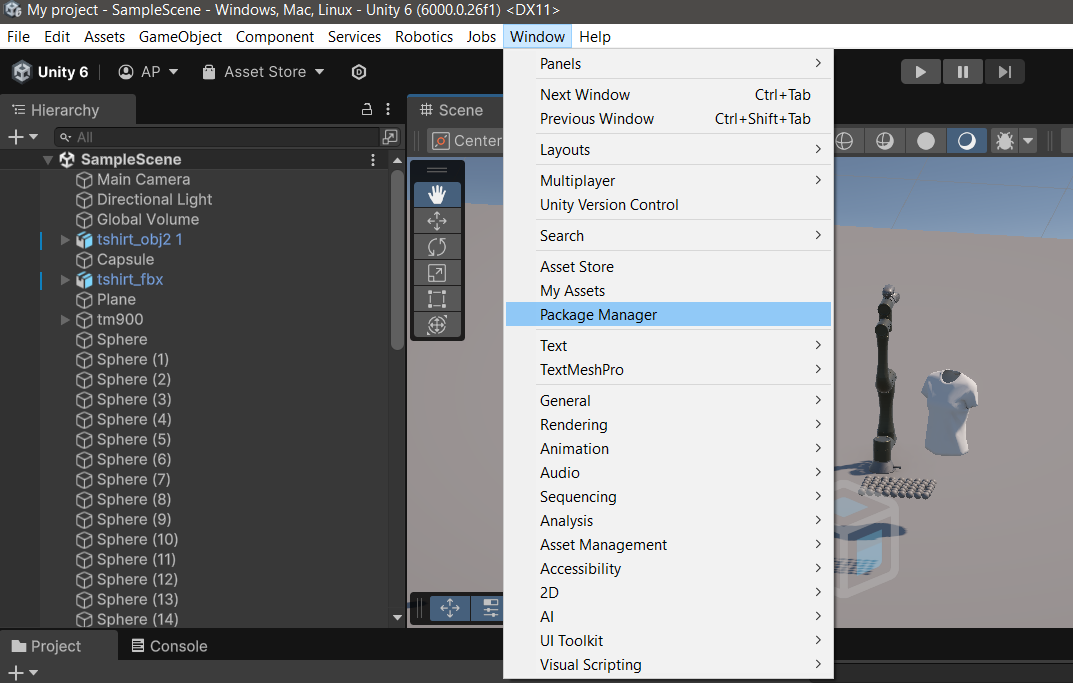
\includegraphics[width=0.4\textwidth]{images/URDF_Importer_1.png}
        \caption{URDF Importer Tutorial}
        \label{fig:URDF_Importer_1}
    \end{figure}
    \item Cliccare su "+" e selezionare "Add package from git URL..."
    \begin{figure}[H]
        \centering
        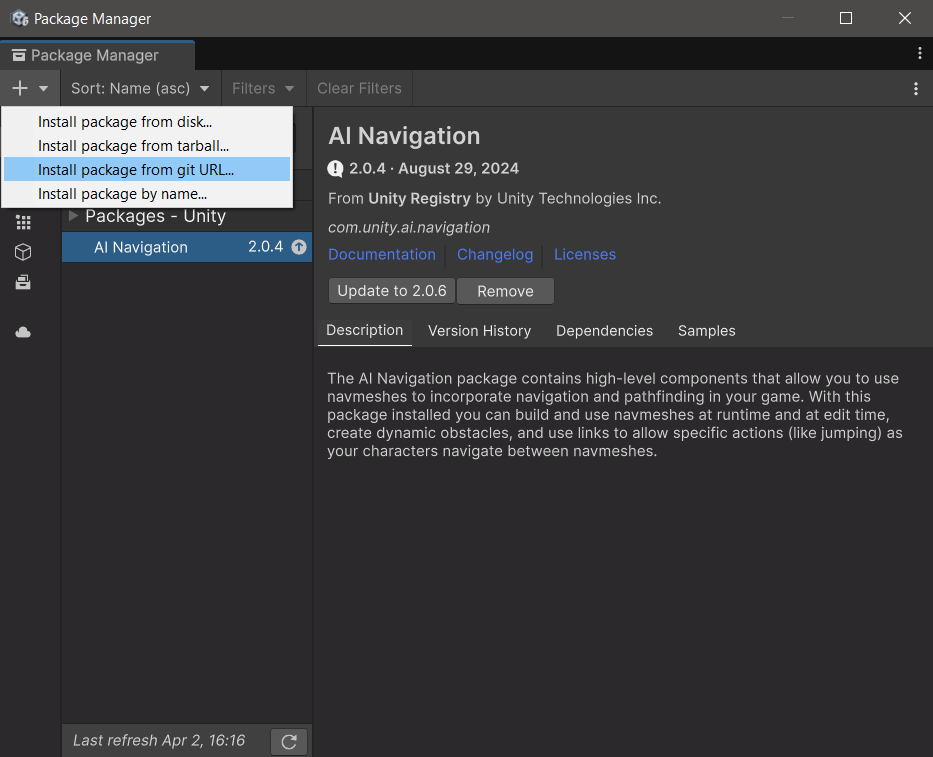
\includegraphics[width=0.4\textwidth]{images/URDF_Importer_2.png}
        \caption{URDF Importer Tutorial}
        \label{fig:URDF_Importer_2}
    \end{figure}
    \item Inserire il seguente URL della repository: 
    \url{https://github.com/Unity-Technologies/URDF-Importer.git} e cliccare "install" per avviare l'installazione
    \begin{figure}[H]
        \centering
        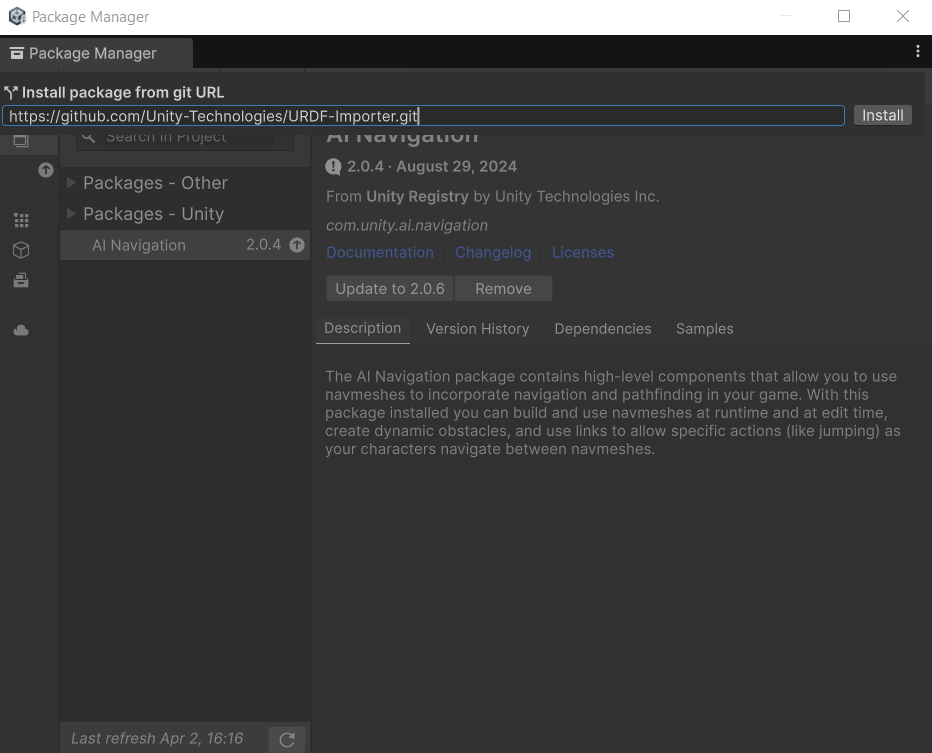
\includegraphics[width=0.4\textwidth]{images/URDF_Importer_3.png}
        \caption{URDF Importer Tutorial}
        \label{fig:URDF_Importer_3}
    \end{figure}
\end{itemize}

Per importare il modello URDF su Unity invece:
\begin{itemize}
    \item Importare il file URDF e le varie mesh sia visual che collision nella cartella "Assets" del progetto Unity
    \begin{figure}[H]
        \centering
        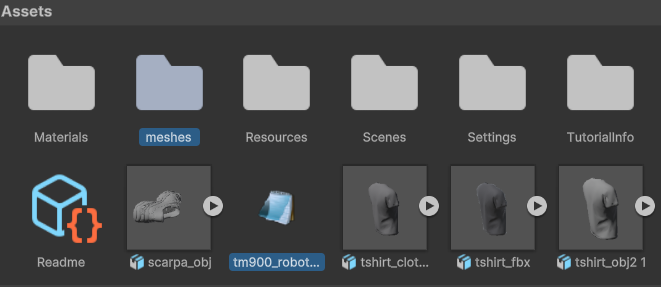
\includegraphics[width=0.5\textwidth]{images/URDF_Importer_4.png}
        \caption{URDF Importer Tutorial}
        \label{fig:URDF_Importer_4}
    \end{figure}
    \item Verificare che i vari path delle mesh all'interno del file URDF siano del tipo ""package://path/delle/meshes" come mostrato in figura \ref{fig:URDF_Importer_5}
    \begin{figure}[H]
        \centering
        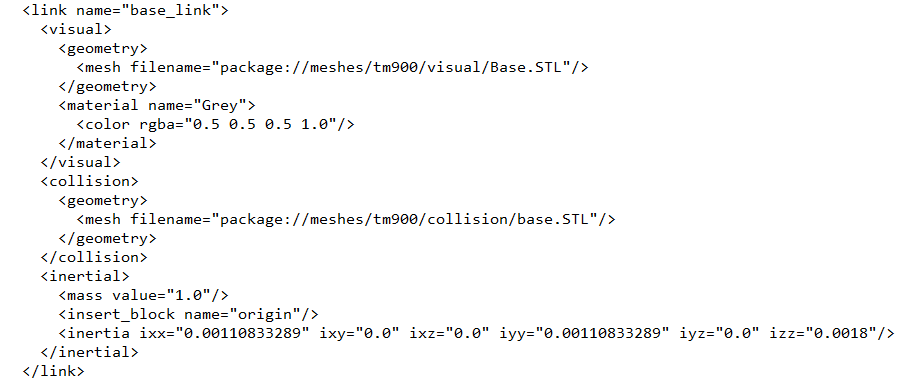
\includegraphics[width=0.5\textwidth]{images/URDF_Importer_5.png}
        \caption{URDF Importer Tutorial}
        \label{fig:URDF_Importer_5}
    \end{figure}
    \item Tasto destro sul file URDF e cliccare su "Import Robot from selected URDF file"
    \begin{figure}[H]
        \centering
        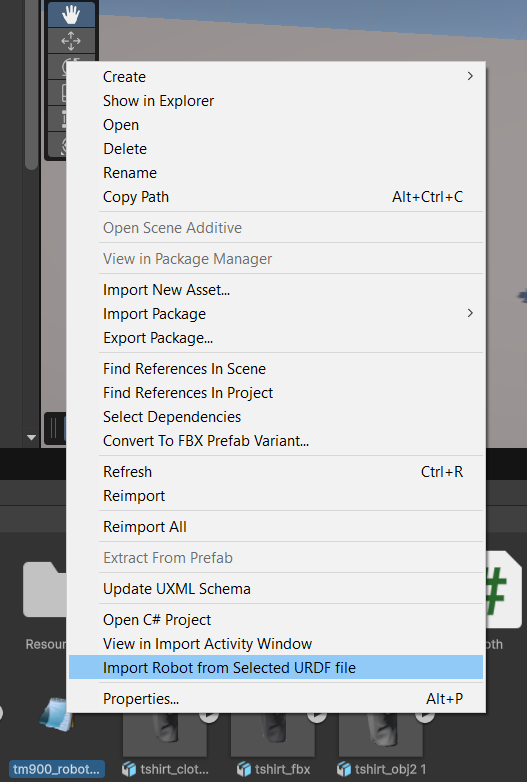
\includegraphics[width=0.35\textwidth]{images/URDF_Importer_6.png}
        \caption{URDF Importer Tutorial}
        \label{fig:URDF_Importer_6}
    \end{figure}
\end{itemize}

A questo punto, se è stato utilizzato il file urdf del TM5-900 corretto, sarà possibile visualizzare il robot come mostrato in figura \ref{fig:URDF_Importer_7}.
\begin{figure}[H]
    \centering
    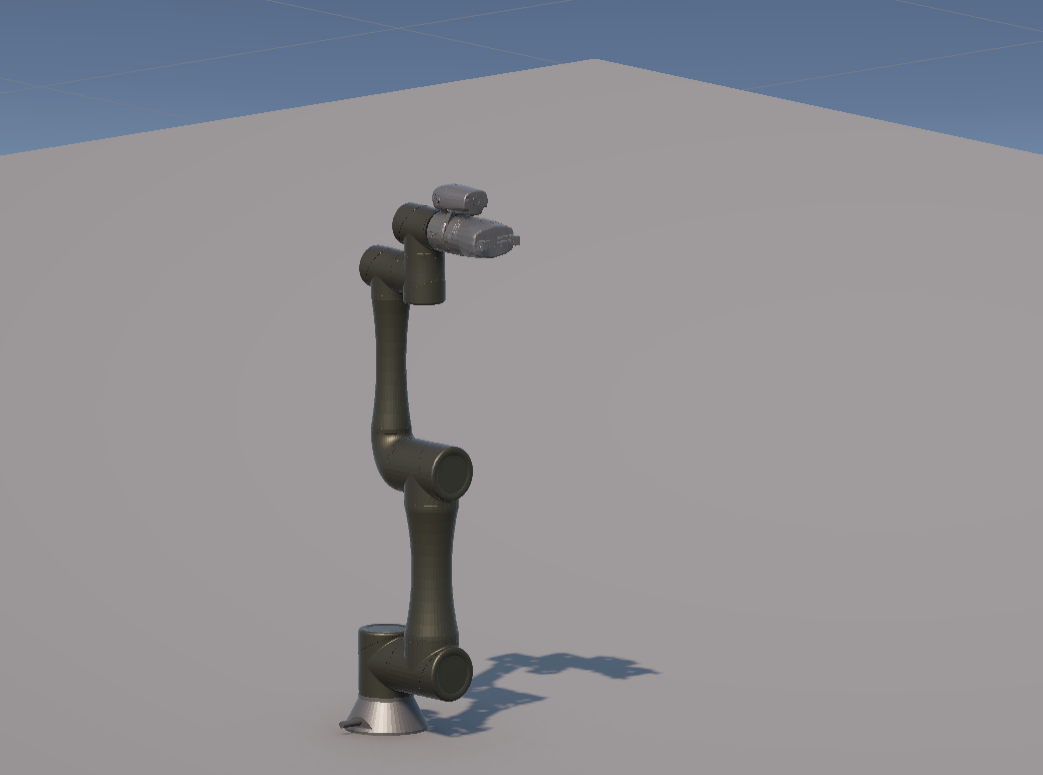
\includegraphics[width=0.35\textwidth]{images/URDF_Importer_7.png}
    \caption{URDF Importer Tutorial}
    \label{fig:URDF_Importer_7}     
\end{figure}

\chapter{Analisi Preliminari e Problematiche Riscontrate}

\section{Problematiche sulle Compatibilità dei Software Utilizzati}

\section{Compatibilità dei File 3D con Unity e Gazebo}

\subsection{Compatibilità dei file con Gazebo e Unity}
Il formato \textbf{.obj} è stato testato con successo sia in Unity che in Gazebo, consentendo l'importazione corretta del modello della t-shirt in entrambi i software. Tuttavia, durante le simulazioni in Unity, l'applicazione del componente Cloth alla t-shirt ha evidenziato alcune difficoltà: il computer ha riscontrato problemi nel gestire correttamente i comandi impostati e, una volta avviata la simulazione, la t-shirt appariva deformata e non realistica, come è possibile vedere nella figura \ref{fig:cloth_error}.

\begin{figure}[h!]
    \centering
    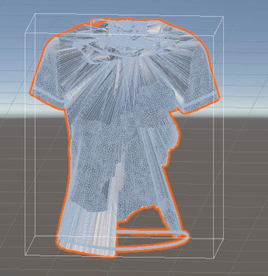
\includegraphics[width=0.4\textwidth]{images/cloth_error.PNG}
    \caption{Errore nell'applicazione del Cloth di Unity}
    \label{fig:cloth_error}
\end{figure}

Per risolvere questo problema, l'oggetto è stato importato nel software Blender, dove è stato utilizzato il modificatore Decimate per ridurre il numero di poligoni della mesh. Diminuendo il parametro "Ratio" a un valore che ha portato la mesh a circa 5000 poligoni, è stato possibile reimportare l'oggetto in Unity e applicare correttamente il componente Cloth, ottenendo una simulazione più realistica.

\begin{figure}[h!]
    \centering
    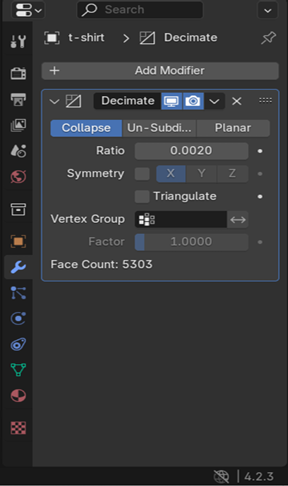
\includegraphics[width=0.3\textwidth]{images/blender_ratio.PNG}
    \caption{Modifica della Mesh nel software Blender}
    \label{fig:blender_ratio}
\end{figure}

Il formato \textbf{.fbx} non è supportato da Gazebo; tuttavia, è compatibile con Unity e può essere convertito in altri formati, come .obj o .dae (Collada), utilizzando Blender. Seguendo lo stesso procedimento adottato per il file .obj, quindi riducendo il numero di poligoni delle mesh tramite il modificatore Decimate in Blender, la simulazione in Unity è stata eseguita correttamente.

Il formato  \textbf{.dae} (Collada) è supportato da Gazebo e risulta essere ampiamente utilizzato in questo contesto. Importando i file .obj della t-shirt e della scarpa, nonché il file .fbx della t-shirt in Blender, è stato possibile esportarli nel formato .dae. Questa operazione ha permesso di caricare correttamente i vari modelli in Gazebo, facilitando la simulazione degli indumenti nel simulatore.

In sintesi, l'utilizzo combinato di Blender per l'ottimizzazione delle mesh e la conversione dei formati, insieme all'applicazione del componente Cloth in Unity, ha consentito di ottenere simulazioni più realistiche del comportamento dei tessuti, migliorando l'interazione tra il robot e gli indumenti nel contesto del progetto.

\subsection{Componente Cloth e collisioni con altri materiali}
Il Cloth di Unity oltre a realizzare una buona fisica per la maglietta è in grado di creare delle collisioni con altri materiali. In particolare, come è stato descritto nel capitolo precedente, si può inserire un oggetto Capsule o Sphere nel Cloth e quindi specificare alla maglietta quali e quanti oggetti dovranno avere un'interazione fisica opportuna durante la collisione. Tuttavia non è possibile far si che l'oggetto a cui è applicato il Cloth (in questo caso la maglietta) collida con un qualunque oggetto di qualunque forma geometrica. Infatti come anticipato è possibile utilizzare solo due tipi di oggetti 3D Unity: Capsule e Sphere. Questa restrizione rappresenta una problematica nel caso in cui il tessuto debba interagire con superfici piatte, angoli o forme geometriche più complesse, come un tavolo, una scatola o una struttura irregolare. Nel caso del progetto un'applicazione utile sarebbe quella di poter far interagire la maglietta con l'end effector del robot che poi riesca ad appoggiarla su una superficie piana come un tavolo. Poiché non è possibile definire direttamente colliders di tipo Mesh o Box per il Cloth, è necessario trovare soluzioni alternative per ottenere un comportamento realistico nelle simulazioni.
\newline
Una soluzione consiste nel posizionare una griglia di piccole Sphere Colliders sulla superficie con cui il tessuto deve interagire. In questo modo, il tessuto percepirà la presenza di una superficie continua, pur utilizzando solo colliders sferici. Per implementare questa soluzione:
\begin{itemize}
\item Creare uno script che generi automaticamente una matrice di sfere sulla superficie desiderata.
\item Assicurarsi che le sfere vengano generate prima che il Cloth venga configurato, in modo che possano essere assegnate correttamente ai "Sphere Colliders" della maglietta.
\item Ottimizzare il numero e la dimensione delle sfere per ottenere una buona resa senza sovraccaricare il motore fisico.
\end{itemize}
\chapter{Struttura del workspace ROS2}

\chapter{Test Effettuati e Risultati Ottenuti}

\chapter{Conclusioni}

\section{Movimentazioe TM5-900 tramite Moveit}
Introduzione a MoveIt
\textbf{MoveIt} è una delle librerie più utilizzate per la pianificazione del movimento in ROS. Consente di controllare bracci robotici, eseguire pianificazioni di traiettoria, gestire collisioni e implementare strategie di manipolazione avanzate. Grazie alla sua integrazione con ROS 2, MoveIt permette di generare e simulare movimenti in modo efficiente, facilitando l'implementazione di algoritmi di pianificazione e controllo.

MoveIt utilizza il modello del robot descritto tramite URDF per comprendere la struttura cinematica del sistema e genera automaticamente il corrispettivo SRDF (Semantic Robot Description Format) contenente la generazione di movimenti validi evitando collisioni. Il suo framework è composto da diversi moduli, tra cui:
\begin{itemize}
    \item Motion Planning: per la generazione di traiettorie.
    \item Collision Checking: per evitare urti tra il robot e l'ambiente.
    \item Kinematic Solvers: per calcolare i movimenti articolari necessari a raggiungere una determinata posizione.
    \item Trajectory Execution: per inviare comandi al robot fisico o alla simulazione.
\end{itemize}

Nel nostro progetto, MoveIt è stato utilizzato per generare i file necessari alla movimentazione del robot TM5-900. In particolare, è stato impiegato lo strumento \textbf{MoveIt Setup Assistant}, che ha permesso di:
1. Importare l'URDF del robot: il modello 3D e la cinematica del TM5-900 sono stati letti direttamente dal file URDF.
2. Generare il file SRDF: che definisce i gruppi cinematici, i giunti, i link e le configurazioni di pianificazione.
3. Configurare i plugin di controllo: per connettere MoveIt a ROS 2 e inviare comandi al robot.
4. Definire le aree di collisione: per garantire che il robot si muova senza urtare gli ostacoli.
5. Generare automaticamente i pacchetti di configurazione: che includono i parametri per il controllo e la simulazione del TM5-900.

Grazie a questa configurazione, MoveIt è stato in grado di elaborare e inviare traiettorie di movimento al robot sia nella simulazione in Unity che in ROS 2.

Applicazione: Definizione di Pose e Simulazione in Unity

Dopo la configurazione iniziale, il nostro obiettivo è stato quello di definire due pose specifiche per il TM5-900 e inviarle alla simulazione in Unity. Il processo seguito è stato il seguente:

1. **Definizione delle pose**: Abbiamo selezionato due posizioni target per il braccio robotico, specificando le coordinate spaziali e gli angoli dei giunti.
2. **Utilizzo di MoveIt per calcolare la traiettoria**: MoveIt ha generato una traiettoria valida evitando collisioni.
3. **Invio dei comandi a ROS 2**: La traiettoria calcolata è stata inviata al nodo ROS 2 responsabile del controllo del robot.
4. **Simulazione in Unity**: I dati di movimento sono stati trasmessi a Unity, dove il modello del TM5-900 si è mosso in base ai comandi ricevuti.

Grazie a questo workflow, siamo riusciti a controllare il robot in modo realistico, testando la movimentazione prima di applicarla in un ambiente reale. L'integrazione tra MoveIt, ROS 2 e Unity ha reso possibile una simulazione efficace, permettendoci di validare il comportamento del TM5-900 prima della sua implementazione fisica.


\section{Importazione TM5-900 in Gazebo}

\section{Camera}

\section{Applicazione finale}

\chapter{Risultati ottenuti e discussione}
% Nell'introduzione al capitolo specificate anche la versione dell'STM32CubeIDE e dell'STM32CubeMX che avete usato (se avete cambiato versione nel corso del progetto mettete l'ultima, quella su cui è sviluppato il codice che consegnate).

% \section{Diagramma di flusso}
% Inserire un diagramma di flusso analogo a quello in Figura \ref{fig:diagramma} che spiega il funzionamento generale del codice sviluppato. Inserire anche una descrizione testuale del funzionamento.

% \begin{figure}[H]
% \centering
% 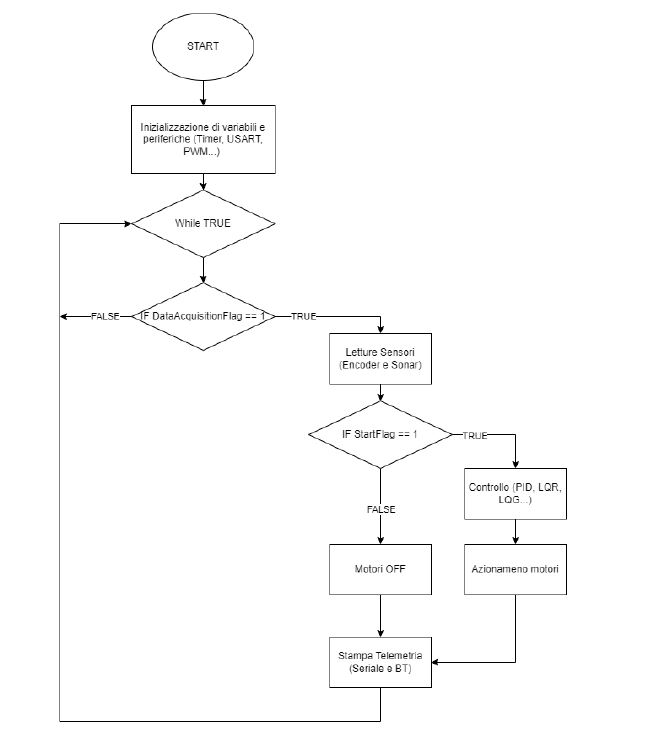
\includegraphics[width=0.8\textwidth,keepaspectratio]{figures/diagramma.JPG}
% \caption{Diagramma di flusso del codice sviluppato}
% \label{fig:diagramma}
% \end{figure}

% \section{Gestione singoli componenti}
% Dedicare un pagagrafo ad ogni componente in cui viene spiegato il codice che lo gestisce. Inserite prima una descrizione generale di come si gestisce un componente di quel tipo (aiutandovi con schemi o altro). Poi le configurazioni che sono state fatte sul .ioc per poterlo utilizzare (quale periferiche sono state abilitate, come sono state configurate.. mettete degli screen del .ioc). Infine inserite e spiegate le parti di codice che lo gestiscono.\\
% \newline
% \textcolor{red}{NOTA per il codice}: per rendere il codice modulare e riutilizzabile è buona prassi non caricare troppo il main ma creare una libreria per ogni componente. Quindi il componente1 avrà un header file "componente1.h" e un source file "componente1.c", nel source file sono implementate le funzioni che gestiscono il componente, nell'header file ci sono i prototipi di tali funzioni in modo che esse possano essere usate nel main includendolo.\\
% \newline
% \textcolor{red}{NOTA per il codice}: non inserire mai nel codice dei parametri numerici senza contesto ma renderli delle costanti definite (usando la direttiva \%define). Se sono delle costanti relative ad uno specifico componente vanno inserite nel relativo header file.\\
% \newline
% \textcolor{red}{NOTA per il codice}: per inserire il codice, anziché utilizzare screenshot utilizzate i seguenti comandi.\\
% Per codice scritto in latex (con linguaggio Python):
% \begin{lstlisting}[language=Python, caption="Codice in Python"]
% import numpy as np
    
% def incmatrix(genl1,genl2):
%     m = len(genl1) # The length of the first array
%     n = len(genl2) # The length of the second array
%     sum = 0
    
%     # Compute 
%     for i in range(0,n):
%         for j in range(0, m):
%             sum += genl1[n]*genl2[m]

%     # Print
%     print("The sum is %2d" %(sum))   
    
%     return M
% \end{lstlisting}
% Per codice richiamato da file (con linguaggio C):

% \lstinputlisting[language=Cpp, firstline=4, lastline=8, caption="Codice in C"]{codefiles/example_code.cpp}

% Funziona anche per codice MATLAB:
% \begin{lstlisting}[language=MATLABc, caption="Codice in MATLAB"]
% %% PREPARE WORKSPACE
% close all
% clearvars
% clc

% %% OPERATIONS
% sayhello;

% %% FUNCTIONS
% function sayhello
%     fprintf("Hello world!");
% end

% \end{lstlisting}


% \subsection{Gestione componente1}

% \subsection{Gestione componente2}

% \section{Funzionamento complessivo}
% Dopo aver spiegato il codice che gestisce i singoli componenti, inserire e commentare le porzioni di codice relative al funzionamento complessivo del programma.

\chapter{Conclusioni e prospettive future}
% Dedicate un capitolo a tutti i test effettuati con relativi risultati, includete sia i test finali relativi al funzionamento complessivo, sia i test delle singole parti (se significativi). \\
% Descrivete in dettaglio le condizioni in cui sono stati svolti i test in modo che siano ripetibili. Durante i test fate dei video e acquisite i dati (es usando la funzione di log di Putty), per i test più rilevanti è opportuno consegnare anche questo materiale per documentare i test effettuati. Nella relazione riportate i risultati con dei grafici come quello in Figura \ref{fig:grafico} (inserite sempre nei grafici le label sugli assi con grandezza e relativa unità di misura). Commentate in modo critico i risultati ottenuti, evidenziando sia quelli positivi sia quelli negativi. 

% \begin{figure}[H]
% \centering
% 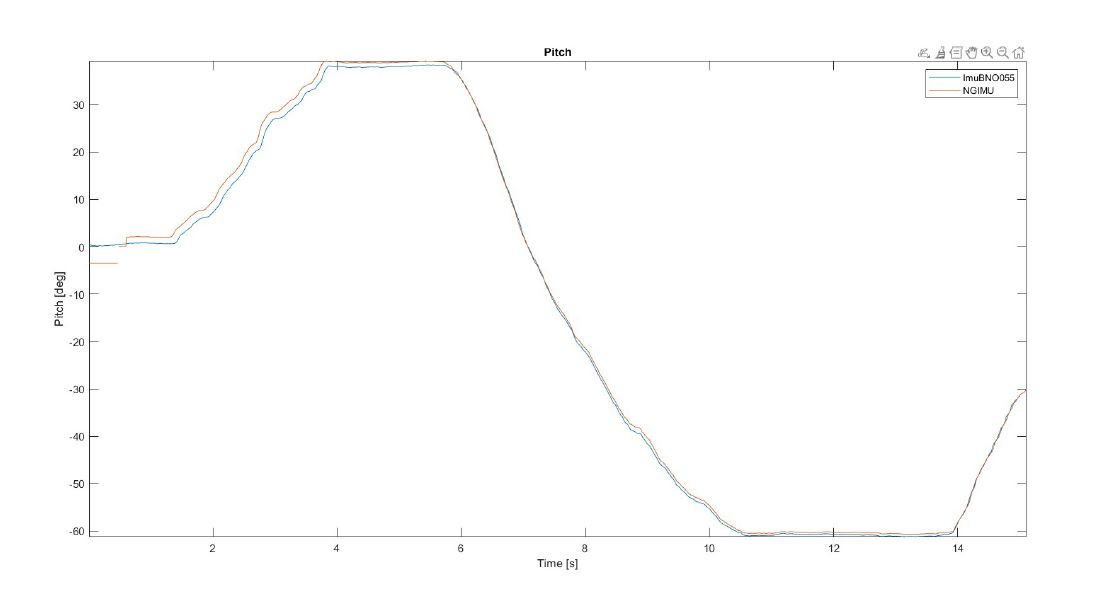
\includegraphics[width=0.8\textwidth,keepaspectratio]{figures/grafico.JPG}
% \caption{Esempio di grafico}
% \label{fig:grafico}
% \end{figure}
% \section{Test1}
% Per ogni test riportate: cosa state testando, in che condizioni si è svolto il test, riferimenti a video/file di log che consegnate insieme a relazione e codice, grafici dei risultati, commento dei risultati.

% \section{Test2}

% \newpage
% \addcontentsline{toc}{chapter}{Conclusioni e sviluppi futuri}
% \section*{Conclusioni e sviluppi futuri}
% Riassumere brevemente il lavoro svolto rispetto al task assegnato, evidenziando quali risultati sono stati raggiunti e quali no. Se ci sono aspetti del task non completati spiegare quali sono stati i problemi riscontrati in merito.\\
% Inserire considerazioni personali su possibili sviluppi futuri dell'attività svolta (idee per migliorarla che non avete avuto modo di sperimentare, aspetti che suggerite di approfondire, problemi da risolvere..).

\addcontentsline{toc}{chapter}{Appendici}
\appendix
\chapter{Appendice1}
Se necessario ricorrete alle appendici per spiegare le parti "di contorno" dell'attività svolta e/o ciò che non riuscite ad inserire nello schema generale dei capitoli della relazione (es acquisizione dei dati con Matlab).


\bibliographystyle{ieeetr}
\bibliography{bibl} 
\end{document}
